\documentclass[fleqn,reqno,10pt]{article}
\usepackage{amsmath}
\usepackage{amsfonts}
\usepackage{amsthm}
\usepackage{amssymb}
\usepackage{mathrsfs}
\usepackage{nicefrac}
%\usepackage{stmaryrd}
%\usepackage{multicol}
\usepackage{graphicx}
\usepackage{color}
\usepackage{booktabs}
\usepackage{pgfplots}
\usepackage{subcaption}

\usepackage{blkarray}
\usepackage{xspace}

\usepackage{tgtermes}
\renewcommand{\baselinestretch}{1.2}

\newcommand{\mylang}[1]{\ensuremath{L_{\text{#1}}}\xspace} %meaningful states
\newcommand{\mystate}[1]{\ensuremath{\state_{\text{#1}}}\xspace} %meaningful states
\newcommand{\mymessg}[1]{\ensuremath{\messg_{\text{#1}}}\xspace} %meaningful messages
\newcommand{\messg}{\ensuremath{m}\xspace}		% single messages
\newcommand{\state}{\ensuremath{s}\xspace}		% single states

\newcommand{\Lbound}{\mylang{bound}}
\newcommand{\Llack}{\mylang{lack}}
\newcommand{\ssome}{\mystate{\ensuremath{\exists\neg\forall}}}
\newcommand{\sall}{\mystate{\ensuremath{\forall}}}
\newcommand{\snone}{\mystate{\ensuremath{\emptyset}}}
\newcommand{\msome}{\mymessg{some}}
\newcommand{\mall}{\mymessg{all}}


\definecolor{mygray}{cmyk}{0.35,0.35,0.35,0.35}
\newcommand{\mygray}[1]{{\textcolor{mygray}{#1}}}


\title{Notes on presentation of model for co-evolution}
\author{Thomas Brochhagen}
\date{}

\begin{document}
\maketitle

\subsection*{Motivation}

We would like to present our model in a cleaner and more intuitive way. As suggested by Michael, one way to do so is to focus first on a reduced type space to illustrate how the model works. As a reminder:

\begin{align*}
  \Lbound & = \begin{blockarray}{lcc}
    & \mygray{\msome} & \mygray{\mall} \\
    \begin{block}{l[cc]}
      \mygray{\ssome} & 1 & 0 \\
      \mygray{\sall}  & 0 & 1 \\
    \end{block}
  \end{blockarray} &
  \Llack & = \begin{blockarray}{lcc}
    & \mygray{\msome} & \mygray{\mall} \\
    \begin{block}{l[cc]}
      \mygray{\ssome} & 1 & 0 \\
      \mygray{\sall}  & 1 & 1 \\
    \end{block}
  \end{blockarray}
\end{align*}

These two lexica are paired with either level-$0$ {\em literal} behavior, or level-$1$ {\em pragmatic} behavior. Learnability-wise, if there is a bias for simpler semantics (no-upper bound), then the two types with $\Llack$ are favored {\em a priori}. Furthermore, both $\Lbound$ users are indiscernible when it comes to learning; they only differ in their receiver behavior. Utility-wise, literal $\Lbound$ fares slightly better than pragmatic $\Lbound$. If $\lambda$ is sufficiently high, then the difference between pragmatic $\Llack$ and both $\Lbound$ types is almost negligible. We want to visualize how (co-)evolution plays out by comparing four populations of two types each, where each pair of types differs only in (i) signaling behavior, or (ii) lexica:

\begin{enumerate}
  \item literal $\Lbound$ vs. literal $\Llack$;
  \item pragmatic $\Lbound$ vs. pragmatic $\Llack$;
  \item literal $\Lbound$ vs. pragmatic $\Lbound$;
  \item literal $\Llack$ vs. pragmatic $\Llack$.
\end{enumerate}

The other relevant parameters of the model are: soft-max parameter $\lambda$, posterior parameter $l$, sequence length $k$, and bias parameter $c$ (detailed below).

\subsection*{Learning bias}
In the paper, the learners' inductive bias is a function of the complexity of the formulae that types lexicalize. Introducing our measure and applying it only to this small type space is probably not the way to go. For illustratory purposes, we may instead assume that there's an abstract parameter (which we later make concrete using our measure) $c \geq 1$ that regulates how strongly $\Llack$ is preferred over $\Lbound$. In what follows, I assumed this to be $P(L_i) \propto c$ if $L_i$ is $\Llack$ and otherwise $1$. For instance, if we have  a type space with $\tau_i$ as literal $\Lbound$ and $\tau_j$ as pragmatic $\Llack$, then $P(\tau_i) \approx .33$ for $c = 2$. This is just for illustration, of course. We can change this at will. As far as I can see, the reduced type spaced behave in a very predictable manner. I set $c = 2$ for all the plots below.

\subsection*{General remarks}
First, I did not succeed in putting the model in an elegant closed form. The good news is that the type space is small enough so that we don't need to sample anything. In particular, we don't need to sample from speaker probabilities to approximate $Q$ for large $k$; we can look at all possible state-message sequences instead, meaning that we get the same result each time we apply replicator or mutator steps. 

Second, there are some issues with phase-portrait-like representations. The main problem is that I have not (yet?) found an algorithm that succeeds in reliably finding stable points for mutator (or replicator-mutator) steps. 

Third, one of the major disadvantages of the smaller type spaces is that (I fear that) they give the impression that the mutator-step is doing most the work. As shown below, $M(x)$ is very close to $M(RD(x))$. This is not true of the bigger type space, but makes sense in these reduced ones. After all, learning is what differentiates $\Llack$ from $\Lbound$. I'm concerned that these results may give a wrong impression.

Lastly, I think that all the representations I generated have some negative sides (details below). Before improving on them, I thought we should discuss these matters, making use of the fact that their flaws are evident. 

\subsection*{Phase portraits}
\begin{figure}
\centering
\begin{subfigure}{.6\textwidth}
  \centering
  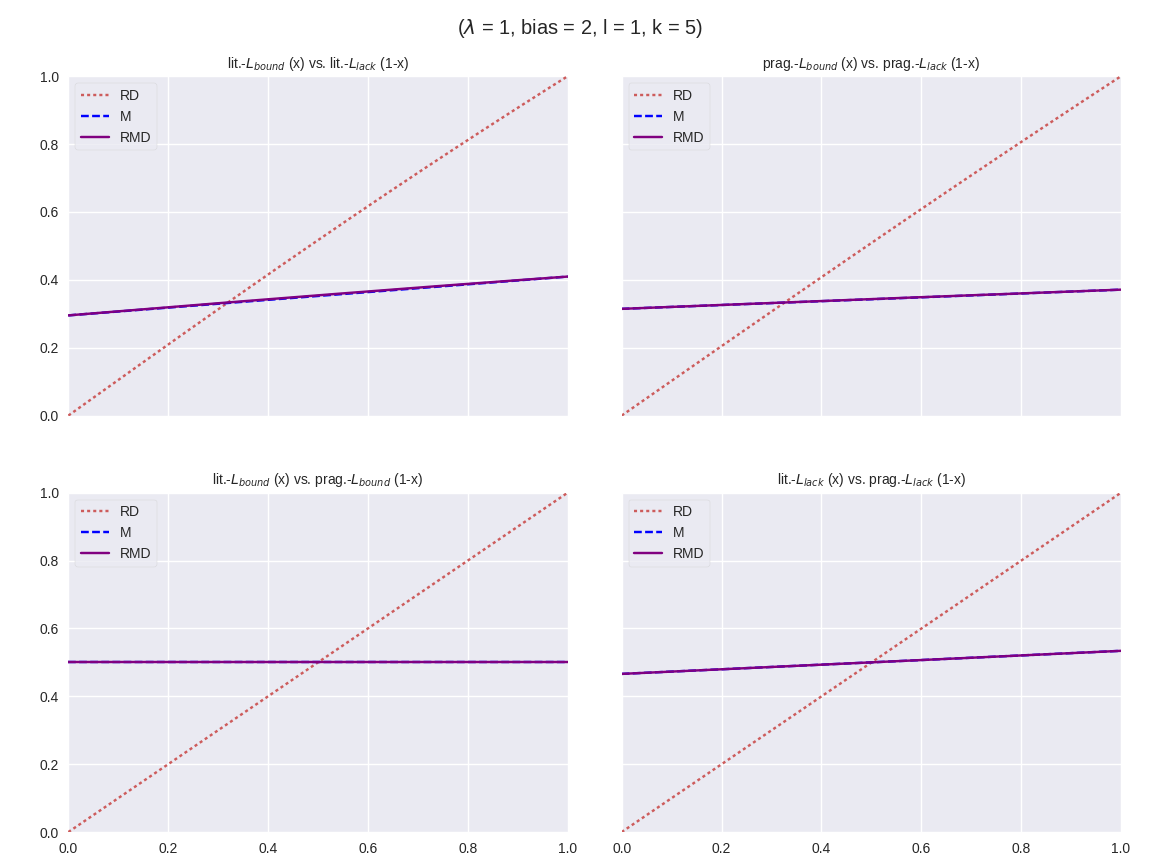
\includegraphics[scale=0.4]{phases-lam01-bias2-l01-k5}
  \caption{}
  \label{fig:sub1}
\end{subfigure}%
\begin{subfigure}{.6\textwidth}
  \centering
  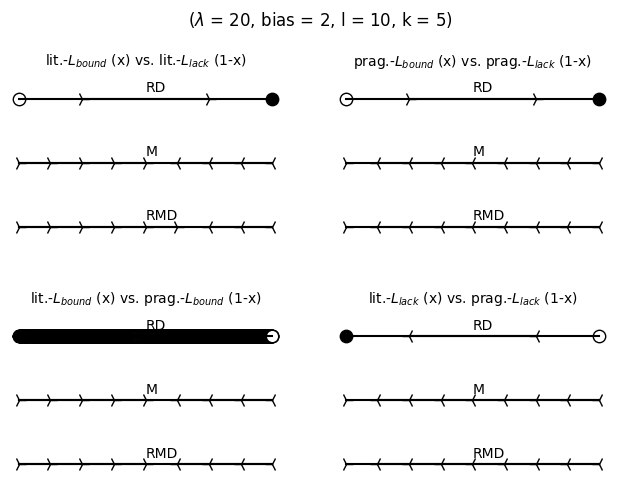
\includegraphics[scale=0.4]{phases-lam20-bias2-l10-k5}
  \caption{}
  \label{fig:sub2}
\end{subfigure}
\caption{Approximate phase-portraits for (a) $\lambda = 1, c = 2, l = 1, k = 5$ and (b) $\lambda = 20, c = 2, l =10, k =5$}
\label{fig:phase}
\end{figure}


Figure \ref{fig:phase} shows $8$ (approximate) portraits for applications of replicator steps only, mutator steps only, and replicator-mutator steps on our four type-pairings, for two parameter constellations. For instance, the upper-left-most portrait shows the dynamics for a type space consisting of literal $\Lbound$ ($x$) and literal $\Llack$ ($1-x$). We can see that, as long as there are some $\Lbound$ types in the population, the population progresses toward the extreme where only this type survives. 

I used a couple of heuristics to generate these plots. First, I took $1000$ points in $[0,1]$ and applied the dynamic in question. Then, I checked if there were any points for which $D(x) = x$. As expected, the only stable points found in this way are the extremes for the replicator step: $RD(1) = 1$ and $RD(0) = 0$. To check whether these points are attractors, I looked at adjacent points to figure out whether they moved toward or away from that point. I did the same for the arrows, evenly spread across the axis.
\begin{itemize}
\item[{\bf The good}] It's easy to see how the dynamics play out. 
\item[{\bf The bad}] It's not easy to find stable points when mutation is involved. As mentioned above, I tried a couple of optimization algorithms but didn't get anywhere so far. Additionally, $M(x)$ and $M(RD(x))$ are (almost) indistinguishable. This is obviously an issue for all the depictions I played around with. It's not as obvious in these ones though.
\item[{\bf The ugly}] There are {\em a lot} of points where $RD(x) = x$ in the type space consisting of only literal and pragmatic $\Lbound$. This explains why these two phase portraits look so ugly; there are many overlapping circles.
\end{itemize}
{\bf My take:} I think these plots are nice but that they require the most cleaning. The major advantage I see here is that, even without finding stable points, it's easy to see where $M(\cdot)$ and $M(RD(\cdot))$ are headed (having less arrows would make this a lot easier to see). This representation slightly masks my big concern of mutator- and RM-steps being almost the same. As for the problem of too many stable points: We could be a little more selective about which points to depict (e.g., relative to the basin of attraction) or use other pictorial means (see the last set of plots).  



\subsection*{Simple plots}
\begin{figure}
\centering
\begin{subfigure}{.6\textwidth}
  \centering
  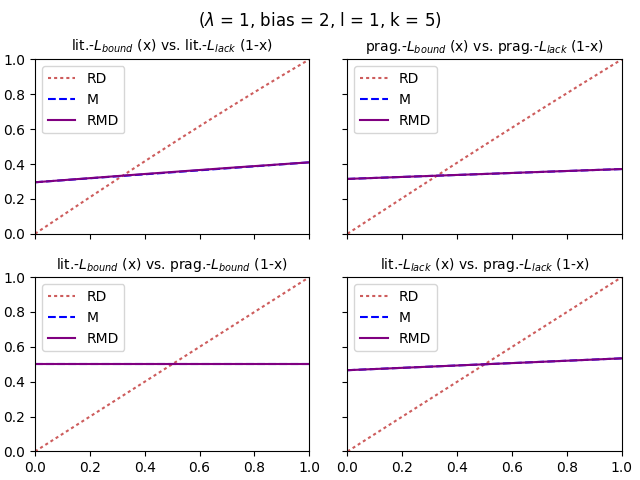
\includegraphics[scale=0.45]{plot-lam01-bias2-l01-k5}
  \caption{}
  \label{fig:sub1}
\end{subfigure}%
\begin{subfigure}{.6\textwidth}
  \centering
  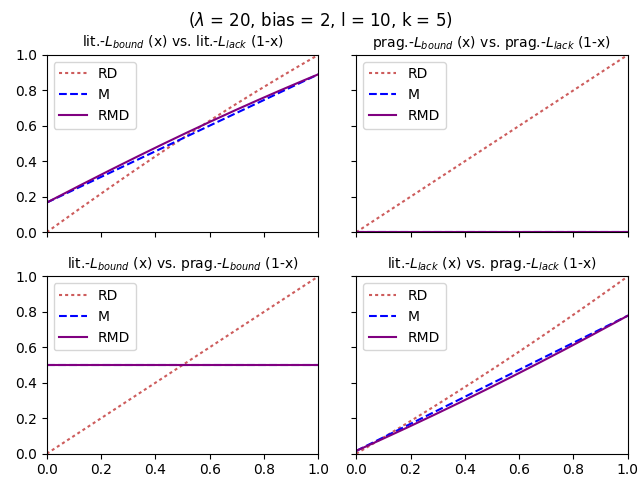
\includegraphics[scale=0.45]{plot-lam20-bias2-l10-k5}
  \caption{}
  \label{fig:sub2}
\end{subfigure}
\caption{Evolutionary competition between pairs of types with (a) $\lambda = 1, c = 2, l = 1, k = 5$ and (b) $\lambda = 20, c = 2, l =10, k =5$. The $x$-axis shows proportion of $x$ before the update, the $y$-axis shows the result of a step of the dynamic on this $x$-value.}
\label{fig:plots}
\end{figure}


Figure \ref{fig:plots} shows $8$ plots using the same data as above. The main difference is that there's no information about stable points and that the directionality of change, particularly in the case of replication only, is harder to see.

\begin{itemize}
\item[{\bf The good}] It's very easy to see the effects of mutation only and the RMD. In particular, that (i) all of $Q$'s cells are equal to $.5$ in populations of only literal and pragmatic $\Lbound$, (ii) but that there is a clear difference in the learnability of literal and pragmatic $\Llack$ due to differences in their likelihoods when $\lambda > 1$.
\item[{\bf The bad}] It's not evident that there are differences across applications of the replicator step. Additionally, these plots may give the impression that replication {\em in general} is doing very little. Particularly when it comes to a comparison between $M(x)$ and $RMD(x)$. I must concede that it is true that replication is doing very little in these reduced type spaces.
\end{itemize}

{\bf My take:} I don't think that we should use plots like these as they don't serve the illustrative purpose we're after. I included them because they clarified a lot of questions I had when I first looked at the phase portraits. 


\subsection*{Dynamics}
\begin{figure}
\centering
\begin{subfigure}{.6\textwidth}
  \centering
  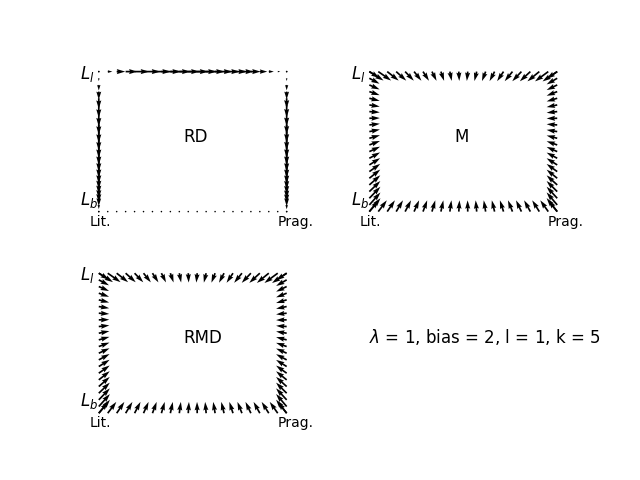
\includegraphics[scale=0.45]{quiver-lam1-c2-k5-l1}
  \caption{}
  \label{fig:sub1}
\end{subfigure}%
\begin{subfigure}{.6\textwidth}
  \centering
  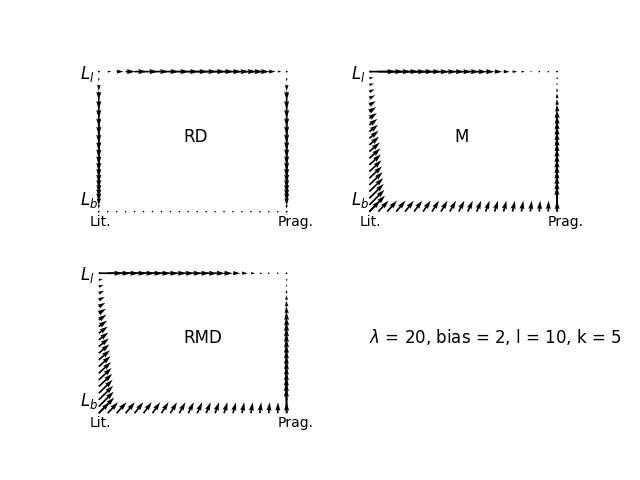
\includegraphics[scale=0.45]{quiver-lam20-c2-k5-l10}
  \caption{}
  \label{fig:sub2}
\end{subfigure}
\caption{Evolutionary competition between pairs of types with (a) $\lambda = 1, c = 2, l = 1, k = 5$ and (b) $\lambda = 20, c = 2, l =10, k =5$. Coordinates $(x,y)$ show (proportion of pragmatic types, proportion of $\Llack$ types).}
\label{fig:quiver}
\end{figure}

Lastly, I wanted to try my hand at compressing the information more while trying to highlight the main take away of the dynamics applied to these reduced type spaces. Figure \ref{fig:quiver} is an illustration. I used the sketch Michael sent us with his comments as inspiration. We think of the type space as being $2$ dimensional. Along the four edges we have same types competing as we had in the previous plots. This $2D$ space is ambiguous once you move from the edges, so I only applied the dynamics on edges. More precisely, in each plot, the $x$-coordinate indicates the proportion of literal types and the $y$-coordinate indicates the proportion of $\Llack$ users. Points that are not on edges are ambiguous because, e.g., $(.5,.5)$ could mean $50\%$ are literal $\Lbound$ and $50\%$ are pragmatic $\Llack$ but also that there are $25\%$ of each of the four types in the population. The edges are unambiguous because each population consists of maximally two types, opposed with respect to a single dimension. This explains why replication in Figure \ref{fig:quiver} only moves along edges.

\begin{itemize}
\item[{\bf The good}] These plots look very similar to what Michael sketched out by hand. The RD plots are also a lot cleaner than the phase portraits I made above.
\item[{\bf The bad}] The ambiguity of $(x,y)$ away from edges.
\item[{\bf The ugly}] Its painfully evident that mutation steps and RMD steps are almost identical. Additionally, vectors are not scaled. Right now, they are automatically resized relative to the other vectors on their edge. This makes it easier to show small effects. If I scale the vectors then the RD plots look as if they consisted only of points because the mutator-steps are much larger. Note also that the movement from pragmatic $\Lbound$ to literal $\Lbound$ under replication only is only apparent when we look at enough points along the edge. However, this makes the plots look cluttered everywhere else. This is fixable and mostly cosmetic though.
\end{itemize}
{\bf My take:} I like these the most. Of course, we could also generate each edge separately and present them in a format similar to that of phase portraits above. 

I couldn't come up with anything, but: Is there a space in which we could disentangle the ambiguity of the $2D$ space? That is, a shape that is as the regular $3$-simplex is to the regular $2$-simplex?




\end{document}
